\documentclass[a4paper,spanish,fixlanguage]{book}
\usepackage[spanish]{babel}
\usepackage[utf8x]{inputenc}
\usepackage[T1]{fontenc}
\usepackage{amsmath,mathtools}    
\usepackage{stmaryrd}
\usepackage[dvipsnames]{xcolor}      %MidnightBlue color in links
\usepackage[resetlabels]{multibib}   %multiple bibliographies
\usepackage[margin=1.55in]{geometry} %page size
%\usepackage{cmbright}                %font
\usepackage{amsthm}                  %theorem styles
\usepackage[spanish]{babelbib}       %bibliografía en español
\usepackage{catchfilebetweentags}    %inclusión de pedazos de código
\usepackage{url}
\usepackage{float}                   %H option in figure
\usepackage[all]{xy}                 %categorical schemas
\usepackage{mathrsfs}
\usepackage{epigraph}
\usepackage{proof}                   %infer, used in exponential.tex
\usepackage{rotating}
\usepackage{latex/agda}
\usepackage[hidelinks]{hyperref}
%\usepackage{changepage}
\usepackage{bookmark}
\usepackage[header]{appendix}
\usepackage{dirtree}                 %directory tree of the appendix
\usepackage{sty/macros}              %macros
\usepackage{sty/unicode}             %unicode characters
\usepackage{sty/prefs}

\usepackage{amsfonts}


%\newcites{Intro}{Referencias hist\'{o}ricas}
%\newcommand{\gitcode}{\url{http://www.github.com/eugeniasimich/containers}}



\begin{document}

\hypersetup{pageanchor=false}
\begin{titlepage}  %Título

	\centering % Centrar
	\scshape % Font linda para las cosas chicas
	
	\textit{\large Facultad de Ciencias Exactas, Ingeniería y Agrimensura - UNR\\Departamento de Ciencias de la Computación }
	
	\vspace{2\baselineskip}
	
	%------------------------------------------------
	%	Título
	%------------------------------------------------
	
	\rule{\textwidth}{1.6pt}\vspace*{-\baselineskip}\vspace*{2pt} % Línea horizontal grande
	\rule{\textwidth}{0.4pt} % Línea horizontal suave
	
	\vspace{\baselineskip} % Espacio pre-título
	
	{\LARGE \textbf{Formalización de mónadas concurrentes en}}
	
	{\LARGE \textbf{Agda: un análisis del caso de la mónada}}

	{\LARGE \textbf{Delay}} % Título
	
	\vspace{0.5\baselineskip} % Espacio post-título
	
	\rule{\textwidth}{0.4pt}\vspace*{-\baselineskip}\vspace{3.2pt} % Línea delgada
	\rule{\textwidth}{1.6pt} % Línea grande
	
	\vspace{3\baselineskip} % Espacio post título
	
	%------------------------------------------------
	%	Subtítulo
	%------------------------------------------------
	
	{\LARGE \textbf{Tesina de Grado}}

	{\Large Licenciatura en Ciencias de la Computación}
	\vspace*{3\baselineskip} % Espaciooo

	
	%------------------------------------------------
	%	Realizadores
	%------------------------------------------------
	
	\Large{\textbf{Autora:}}
	
	%\vspace{0.5\baselineskip} % Espacio
	
    {\itshape\LARGE Bini, Valentina María}
	
	%\vspace{0.5\baselineskip} % Espacio	
	
	%\large{Legajo: B-5926/9}
	
	\vspace{2\baselineskip} % Espacio

        \Large{\textbf{Director:}}
	
	%\vspace{0.5\baselineskip} % Espacio
	
    {\itshape\LARGE Rivas, Exequiel}

	\vspace*{7\baselineskip} %Espacio pre imagen
    
    %Imagen
    \begin{figure}[h] %El h es para que quede en el lugar
	\centering
	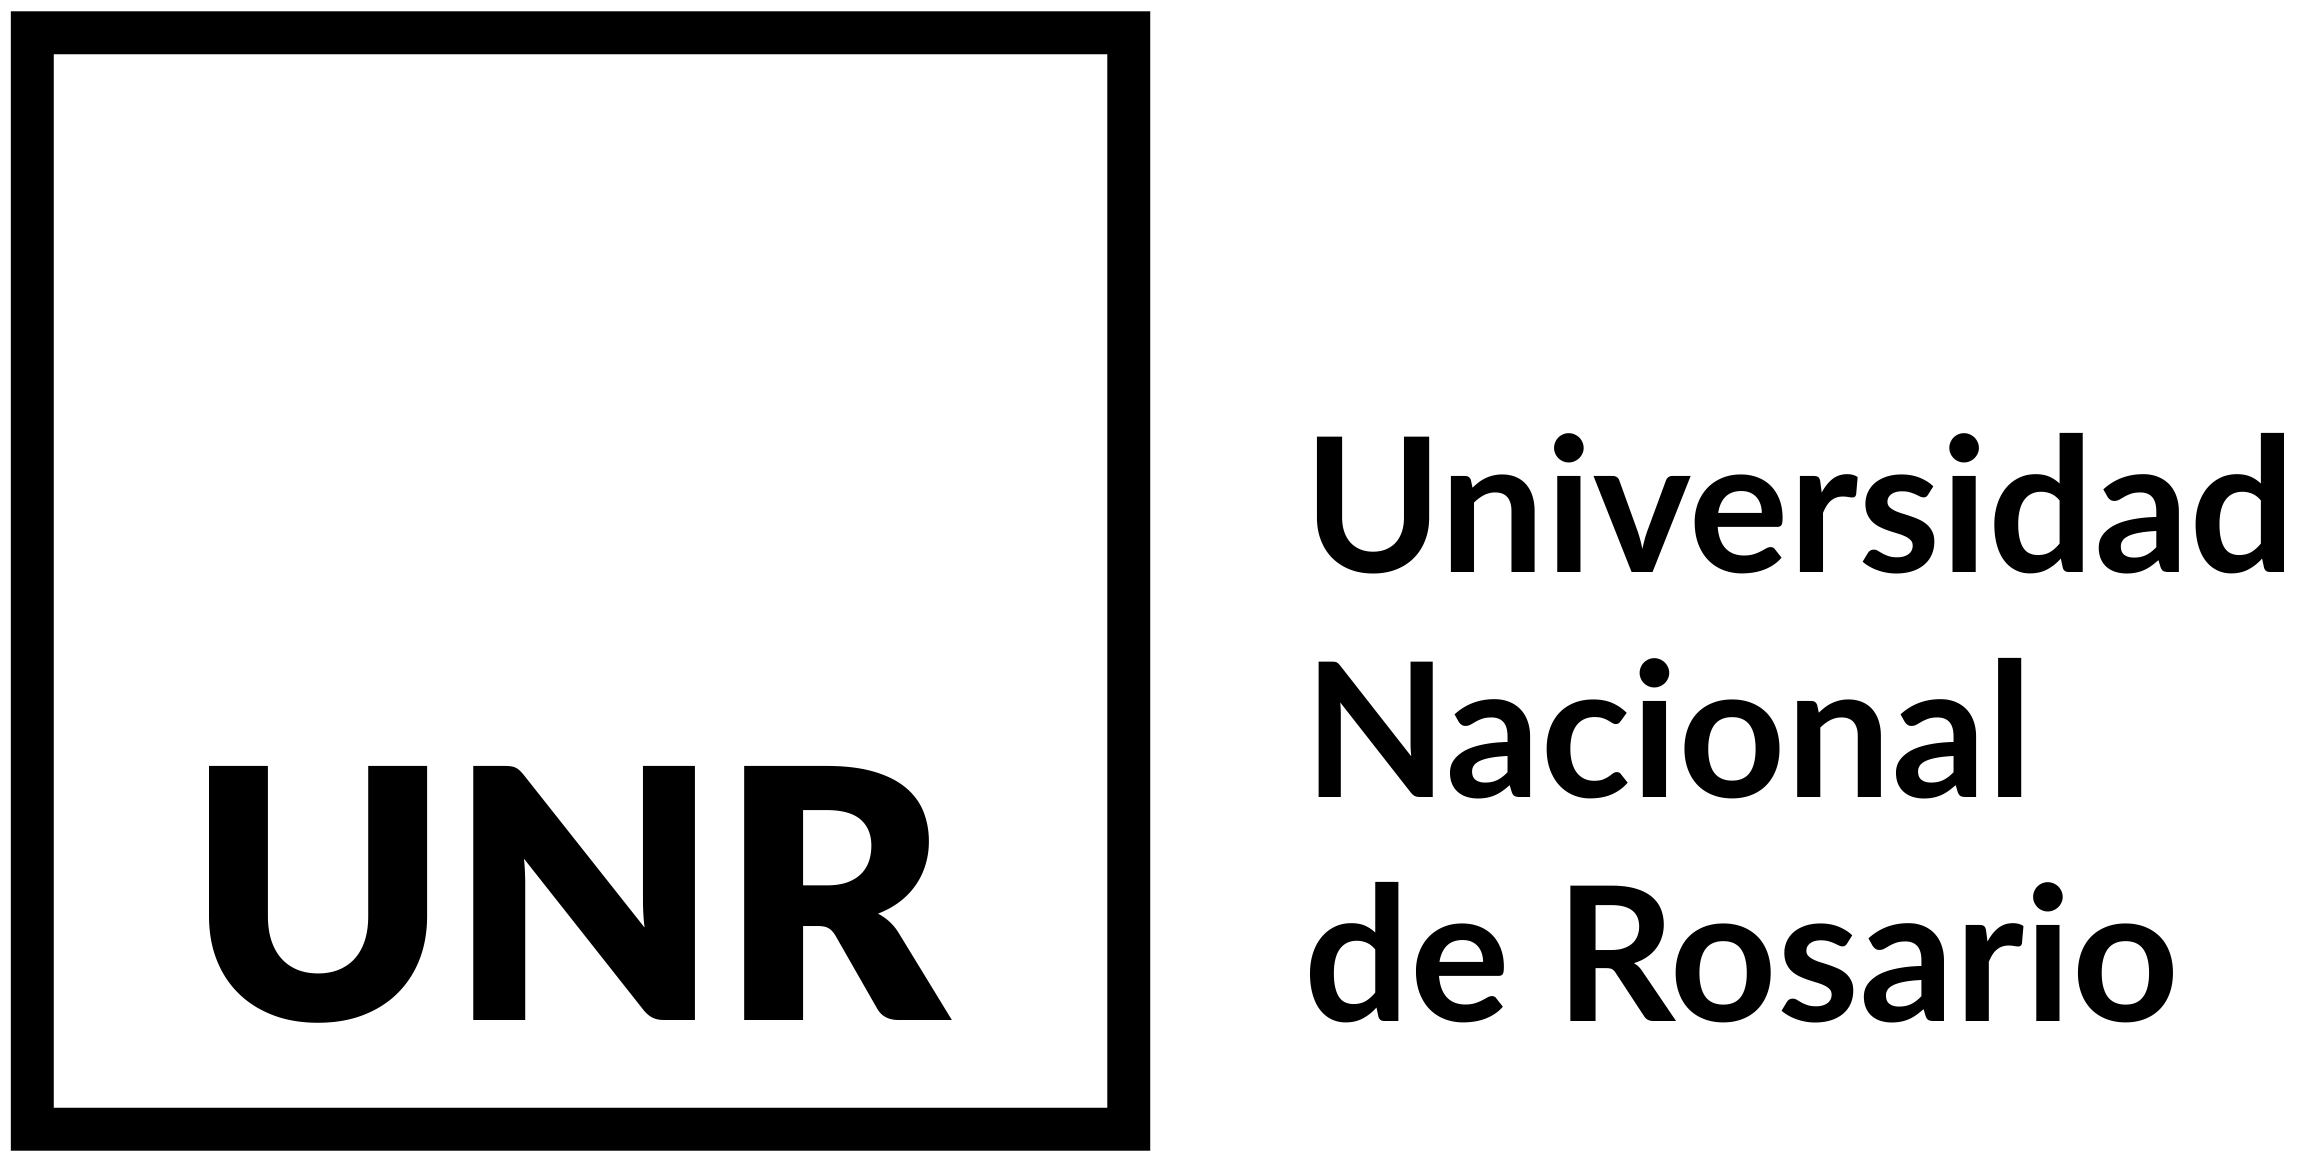
\includegraphics[height=4\baselineskip]{img/UNR.png} \hfill 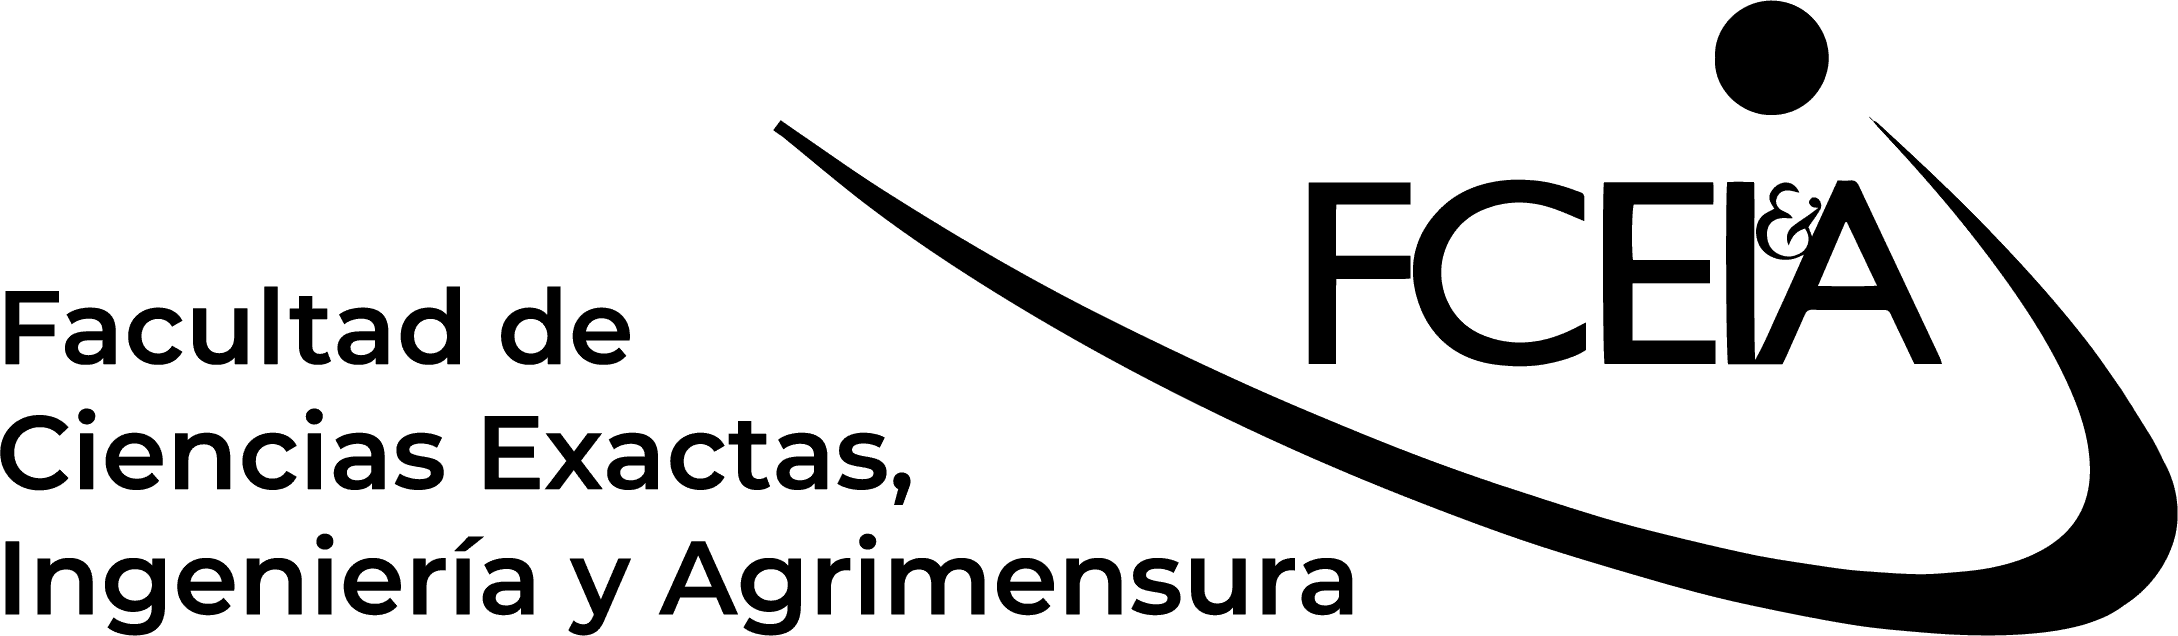
\includegraphics[height=3.7\baselineskip]{img/FCEIA.png} 
	\end{figure}
    
    \vfill % Espacio
	
	%------------------------------------------------
	%	Publicador o fecha
	%------------------------------------------------
		
	\vspace{0.2\baselineskip} % Espacio
	
	%13-12-2022 % Fecha
	

\end{titlepage}


\thispagestyle{empty}

%\chapter*{Resumen}

En los últimos años, la concurrencia ha cobrado mucha importancia en el mundo de la programación, sobre todo debido a la masificación de los procesadores con múltiples núcleos. Los lenguajes de programación funcional, en general, proveen la capacidad de concurrencia mediante funciones \textit{ad-hoc}, y no mediante primitivas bien fundadas del lenguaje. 

Los programas con efectos suelen representarse en los lenguajes de programación funcional mediante el uso de mónadas. Nace entonces el concepto de mónada concurrente en la búsqueda de obtener primitivas bien fundadas para la concurrencia en los lenguajes de programación funcional, extendiendo las mónadas con un nuevo operador: la intercalación de computaciones. La propiedad principal de las mónadas concurrentes es la ley de intercambio, axioma que postula la relación que debe existir entre la secuenciación de computaciones (el operador original \textit{bind}) y el nuevo operador. 
 
La mónada \textit{delay} fue definida con el objetivo de capturar el efecto de la no terminación de programas de manera explícita y uniforme. Los habitantes del tipo \textit{delay} son valores ``demorados'', los cuales pueden no terminar y, por lo tanto, no retornar un valor nunca.

En este trabajo se presenta una formalización del concepto de mónada concurrente en el lenguaje y asistente de pruebas Agda, así como también otras formalizaciones de conceptos previos como las mónadas, los funtores monoidales y los monoides concurrentes. Luego se analiza el caso particular de la mónada \textit{delay}, con el objetivo de probar o refutar que esta puede dotarse de una estructura de mónada concurrente. La principal dificultad que se encontró a la hora de realizar esta prueba es la demostración de la ley de intercambio. Se buscó entonces una simplificación del problema y se demostró que los números conaturales forman un monoide concurrente, obteniendo luego una mónada concurrente alternativa a \textit{delay}: la mónada \textit{writer} con los conaturales como monoide.
%\thispagestyle{empty}

%\frontmatter

\tableofcontents

%\mainmatter

%Intro


\part{Preliminares}

\chapter{Introducci\'on a Agda} \label{chapter:agda}

Agda es un lenguaje de programación funcional desarrollado por la Universidad de Chalmers que se caracteriza por tener tipos dependientes. A diferencia de otros lenguajes donde hay una separación clara entre el mundo de los tipos y el de los valores, en un lenguaje con tipos dependientes estos universos están más entremezclados. Los tipos pueden contener valores arbitrarios (lo que los hace \textit{depender} de ellos) y pueden aparecer también como argumentos o resultados de funciones.

El hecho de que los tipos puedan contener valores, permite que se puedan escribir propiedades de ciertos valores como tipos. Los elementos de estos tipos son pruebas de que la propiedad que representan es verdadera. Esto hace que los lenguajes con tipos dependientes puedan ser utilizados como una lógica. Esta fue la idea principal de la teoría de tipos desarrollada por Martin Löf, en la cual está basado el desarrollo de Agda. Una característica importante de esta teoría es su enfoque constructivista, en el cual para demostrar la existencia de un objeto debemos construirlo.

Para poder utilizar a Agda como una lógica se necesita que sea consistente, y es por eso que se requiere que todos los programas sean totales, es decir que no tienen permitido fallar o no terminar. En consecuencia, Agda incluye mecanismos que comprueban la terminación de los programas.

El objetivo de esta sección es presentar una introducción a Agda, haciendo énfasis en las características necesarias para exponer la temática de esta tesina. 

\section{Tipos de datos y \textit{Pattern Matching}}

Un concepto clave en Agda es el \textit{pattern matching} sobre tipos de datos algebraicos. Al agregar los tipos dependientes el \textit{pattern matching} se hace aún más poderoso. Se verá este tema más en detalle en la sección ??. Para comenzar, en esta sección se describirán las funciones y tipos de datos con tipos simples. 

Los tipos de datos se definen utilizando una declaración \AgdaKeyword{data}, en la que se especifica el nombre y el tipo del tipo de dato a definir, así como los constructores y sus respectivos tipos. En el siguiente código se puede ver una forma de definir el tipo de los booleanos:

\ExecuteMetaData[latex/Agda.tex]{booleans}

El tipo de \AgdaDatatype{Bool} es \AgdaPrimitiveType{Set}, el tipo de los tipos pequeños. Las funciones sobre \AgdaDatatype{Bool} pueden definirse por \textit{pattern matching}:

\ExecuteMetaData[latex/Agda.tex]{not}

Las funciones en Agda no tienen permitido fallar, por lo que una función debe cubrir todos los casos posibles. Esto será constatado por el \textit{type checker}, el cual lanzará un error si hay casos no definidos. 

Otro tipo de dato que puede ser útil son los números naturales. 

\ExecuteMetaData[latex/Agda.tex]{naturals}

La suma sobre números naturales puede ser definida como una función recursiva (también utilizando \textit{pattern matching}). 

\ExecuteMetaData[latex/Agda.tex]{add}

Para garantizar la terminación de la función, las llamadas recursivas deben ser aplicadas a argumentos más pequeños que los originales. En este caso, \AgdaFunction{\_+\_} pasa el chequeo de terminación ya que el primer argumento se hace más pequeño en la llamada recursiva. 

Si el nombre de una función contiene guiones bajos (\AgdaSymbol{\_}), entonces puede ser utilizado como un operador en el cual los argumentos se posicionan donde están los guiones bajos. En consecuencia, la función \AgdaFunction{\_+\_} puede ser utilizada como un operador infijo escribiendo \AgdaArgument{n} \AgdaFunction{+} \AgdaArgument{m} en lugar de \AgdaFunction{\_+\_} \AgdaArgument{n m}. 

La precedencia y asociatividad de un operador se define utilizando una declaración \AgdaKeyword{infix}. Para mostrar esto se agregará, además de la suma, una función producto (la cual tiene más precedencia que la suma). La precedencia y asociatividad de ambas funciones podría escribirse de la siguiente manera:

\ExecuteMetaData[latex/Agda.tex]{precedence}

La palabra clave \AgdaKeyword{infixl} indica que se asocia a izquierda (de igual manera existe \AgdaKeyword{infixr} para asociar a derecha o \AgdaKeyword{infix} si no se asocia hacia ningún lado) y el número que sigue indica la precedencia, operadores con mayor número tendrán más precedencia que operadores con menor número.

\subsection{Tipos de datos parametrizados}

Los tipos de datos pueden estar parametrizados por otros tipos de datos. El tipo de las listas de elementos de tipo arbitrario se define de la siguiente manera:

\ExecuteMetaData[latex/Agda.tex]{lists}


\subsection{Patrones con puntos}

En algunos casos, al definir una función por \textit{pattern matching}, ciertos patrones de un argumento fuerzan que otro argumento tenga un único valor posible que tipe correctamente. Para indicar que el valor de un argumento fue deducido por chequeo de tipos y no observado por \textit{pattern matching},  se le agrega delante un punto (\AgdaSymbol{.}). Para mostrar un ejemplo de uso de un patrón con punto, se considerará el siguiente tipo de dato \AgdaDatatype{Square} definido como sigue:


\ExecuteMetaData[latex/Agda.tex]{square}

El tipo \AgdaDatatype{Square} \AgdaArgument{n} representa una propiedad sobre el número \AgdaArgument{n}, la cual dice
dicho número es un cuadrado perfecto. Un habitante de tal tipo es una prueba de que el número \AgdaArgument{n} efectivamente es un cuadrado perfecto. Si se quisiera definir entonces una función \AgdaFunction{root} que tome un natural y una prueba de que dicho natural es un cuadrado perfecto, y devuelva su raíz cuadrada, podría realizarse de la siguiente manera:

\ExecuteMetaData[latex/Agda.tex]{root}

Se puede observar que al \textit{matchear} el argumento de tipo \AgdaDatatype{Square} \AgdaArgument{n} con el constructor \AgdaFunction{sq} aplicado a un natural \AgdaArgument{m}, \AgdaArgument{n} se ve forzado a ser igual a \AgdaArgument{m} \AgdaFunction{*} \AgdaArgument{m}.


\subsection{Patrones absurdos}

Otro tipo de patrón especial es el patrón absurdo. Usar un patrón absurdo al definir una función significa que no es necesario dar una definición para ese caso ya que no hay manera alguna en la que alguien pudiera dar un argumento para la función. El tipo de dato definido a continuación será de utilidad para ver un ejemplo de este tipo de patrones:

\ExecuteMetaData[latex/Agda.tex]{even}

El tipo \AgdaDatatype{Even} \AgdaArgument{n} representa, al igual que \AgdaDatatype{Square} \AgdaArgument{n}, una propiedad sobre \AgdaArgument{n}. En este caso la propiedad afirma que \AgdaArgument{n} es un número par. Un habitante de este tipo es una prueba de que dicha proposición se cumple. 

Si se quisiera definir una función que, dado un número y una prueba de que es par, devuelva el resultado de dividirlo por dos, podría realizarse de la siguiente manera:

\ExecuteMetaData[latex/Agda.tex]{half}

Se puede ver que en el caso del \AgdaNumber{1}, no existe una prueba de que ese número sea par, y por lo tanto no debemos dar una definición para ese caso. Requerir la pureba de paridad nos asegura que no hay riesgo de intentar dividir por dos un número impar. 

\subsection{El constructor \texttt{with}}

A veces no alcanza con hacer \textit{pattern matching} sobre los argumentos de una función, sino que se necesita analizar por casos el resultado de alguna computación intermedia. Para esto se utiliza el constructor \AgdaKeyword{with}. 

Si se tiene una expresión \AgdaArgument{e} en la definición de una función \AgdaFunction{f}, se puede abstraer \AgdaFunction{f} sobre el valor de \AgdaArgument{e}. Al hacer esto se agrega a \AgdaFunction{f} un argumento extra, sobre el cual se puede hacer \textit{pattern matching} al igual que con cualquier otro argumento. 

Para proveer un ejemplo de uso del constructor \AgdaKeyword{with}, se definirá a continuación la relación de orden \AgdaFunction{\_<\_} sobre los números naturales.

\ExecuteMetaData[latex/Agda.tex]{less}

Si se quisiera definir entonces, utilizando esta función, una función \AgdaFunction{min} que calcule el mínimo entre dos números naturales \AgdaArgument{x} e \AgdaArgument{y}, se debería analizar cuál es el resultado de calcular \AgdaArgument{x} \AgdaFunction{<} \AgdaArgument{y}. Esto se escribe haciendo uso del constructor \AgdaKeyword{with} como sigue:

\ExecuteMetaData[latex/Agda.tex]{min}

El argumento extra que se agrega está separado por una barra vertical y corresponde al valor de la expresión \AgdaArgument{x} \AgdaFunction{<} \AgdaArgument{y}. Se puede realizar esta abstracción sobre varias expresiones a la vez, separándolas entre ellas mediante barras verticales. Las abstracciones \AgdaKeyword{with} también pueden anidarse. En el lado izquierdo de las ecuaciones, los argumentos abstraídos con \AgdaKeyword{with} deben estar separados también con barras verticales. 

En este caso, el valor que tome \AgdaArgument{x} \AgdaFunction{<} \AgdaArgument{y} no cambia nada la información que se tiene sobre los argumentos \AgdaArgument{x} e \AgdaArgument{y}, por lo que volver a escribirlos no es necesario, puede reemplazarse la parte izquierda por tres puntos como se muestra a continuación:

\ExecuteMetaData[latex/Agda.tex]{min2} 

\section{Funciones dependientes}

Como se mencionó anteriormente, una de las principales características de Agda es que tiene tipos dependientes. El tipo dependiente más básico de todos son las funciones dependientes, en las cuales el tipo del resultado depende del valor del argumento. En Agda se escribe \AgdaSymbol{(}\AgdaArgument{x} \AgdaSymbol{:} \AgdaDatatype{A}\AgdaSymbol{)} \AgdaSymbol{$\rightarrow$} \AgdaDatatype{B} para indicar el tipo de una función que toma un argumento \AgdaArgument{x} de tipo \AgdaDatatype{A} y devuelve un resultado de tipo \AgdaDatatype{B}, donde \AgdaArgument{x} puede aparecer en \AgdaDatatype{B}. Un caso especial de esto es cuando \AgdaArgument{x} es un tipo en sí mismo. Se podría definir, por ejemplo:

\ExecuteMetaData[latex/Agda.tex]{id}

\AgdaFunction{identity} es una función dependiente que toma como argumento un tipo \AgdaDatatype{A} y un elemento de \AgdaDatatype{A} y retorna dicho elemento. De esta manera se codifican las funciones polimórficas en Agda. 

A continuación se muestra un ejemplo de una función dependiente menos trivial, la cual toma una función dependiente y la aplica a cierto argumento:

\ExecuteMetaData[latex/Agda.tex]{apply}

\subsection{Argumentos Implícitos}

Los tipos dependientes sirven para definir funciones polimórficas. Pero en los ejemplos provistos en la sección anterior se da de forma explícita el tipo al cual cierta función polimórfica se debe aplicar. Usualmente esto es diferente. En general se espera que el tipo sobre el cual se va a aplicar una función polimórfica sea inferido por el \textit{type checker}. Para solucionar este problema, Agda utiliza un mecanismo de \textit{argumentos implícitos}. 

Para declarar un argumento implícito de una función, se utilizan llaves en lugar de paréntesis. \AgdaSymbol{\{}\AgdaArgument{x} \AgdaSymbol{:} \AgdaDatatype{A}\AgdaSymbol{\}} \AgdaSymbol{$\rightarrow$} \AgdaDatatype{B} significa lo mismo que \AgdaSymbol{(}\AgdaArgument{x} \AgdaSymbol{:} \AgdaDatatype{A}\AgdaSymbol{)} \AgdaSymbol{$\rightarrow$} \AgdaDatatype{B}, excepto que cuando se utiliza una función de este tipo el verificador de tipos intenta inferir el argumento por su cuenta. 

Con esta nueva sintaxis puede definirse una nueva versión de la función identidad, donde no es necesario explicitar el tipo argumento:

\ExecuteMetaData[latex/Agda.tex]{id2} 

Se puede observar que el tipo argumento es implícito tanto cuando la función se aplica como cuando es definida. No hay restricciones sobre cuáles o cuántos argumentos pueden ser implícitos, así como tampoco hay garantías de que estos puedan ser efectivamente inferidos por el \textit{type checker}. 

Para dar explícitamente un argumento implícito se usan también llaves. \AgdaFunction{f} \AgdaSymbol{\{}\AgdaArgument{v}\AgdaSymbol{\}} asigna \AgdaArgument{v} al primer argumento implícito de \AgdaFunction{f}. Si se requiere explicitar un argumento que no es el primero, escribe \AgdaFunction{f} \AgdaSymbol{\{}\AgdaArgument{x} \AgdaSymbol{=} \AgdaArgument{v}\AgdaSymbol{\}}, lo cual asigna \AgdaArgument{v} al argumento implícito llamado \AgdaArgument{x}. El nombre de un argumento implícito se obtiene de la declaración del tipo de la función. 

Si se desea, por el contrario, que el verificador de tipos infiera un término que debería darse explícitamente, se puede reemplazar por un guión bajo. Por ejemplo:

\ExecuteMetaData[latex/Agda.tex]{one'}

\section{Familias de Tipos de datos}



\section{Sistema de Módulos}

El objetivo del sistema de módulos de Agda es manejar el espacio de nombres. Un programa se estructura en diversos archivos, cada uno de los cuales tiene un módulo \textit{top-level}, dentro del cual van todas las definiciones. El nombre del módulo principal de un archivo debe coincidir con el nombre de dicho archivo. Si se tiene, por ejemplo, un archivo llamado \texttt{Agda.agda}, al comienzo del archivo se debería encontrar la siguiente línea:

\ExecuteMetaData[latex/Agda.tex]{module} 

Dentro del módulo principal se pueden definir otros módulos. Esto se hace de la misma manera que se define el módulo \textit{top-level}. Por ejemplo:

\ExecuteMetaData[latex/Agda.tex]{moduleNumbers}

Para acceder a entidades definidas en otro módulo hay que anteponer al nombre de la entidad el nombre del módulo en el cual está definida. Para hacer referencia a \AgdaDatatype{Nat} desde fuera del módulo \AgdaModule{Numbers} se debe escribir \AgdaModule{Numbers.Nat}:


\ExecuteMetaData[latex/Agda.tex]{one}


La extensión de los módulos (excepto el módulo principal) se determina por indentación. Si se quiere hacer referencia a las definiciones de un módulo sin anteponer el nombre del módulo constantemente se puede utilizar la sentencia \AgdaKeyword{open}, tanto localmente como en \textit{top-level}:


\ExecuteMetaData[latex/Agda.tex]{two}


\ExecuteMetaData[latex/Agda.tex]{two2}


Al abrir un módulo, se puede controlar qué definiciones se muestran y cuáles no, así como también cambiar el nombre de algunas de ellas. Para esto se utilizan las palabras clave \AgdaKeyword{using} (para restringir cuáles definiciones traer), \AgdaKeyword{hiding} (para esconder ciertas definiciones) y \AgdaKeyword{renaming} (para cambiarles el nombre). Si se quisiera abrir el módulo \AgdaModule{Numbers} ocultando la función \AgdaFunction{suc₂} y cambiando los nombres del tipo y los constructores, se debería escribir:

\ExecuteMetaData[latex/Agda.tex]{hidingrenaming}

\subsection{Módulos Parametrizados}

Los módulos pueden ser parametrizados por cualquier tipo de dato. En caso de que se quiera definir un módulo para ordenar listas, por ejemplo, puede ser conveniente asumir que las listas son de tipo $A$ y que tenemos una relación de orden sobre $A$. A continuación se presenta dicho ejemplo: 


\ExecuteMetaData[latex/Agda.tex]{sort}


Cuando se mira desde afuera una función definida dentro de un módulo parametrizado, la función toma como argumentos, además de los propios, los parámetros del módulo. De esta manera se podría definir:


\ExecuteMetaData[latex/Agda.tex]{sort1}


También pueden aplicarse todas las funciones de un módulo parametrizado a los parámetros del módulo de una vez instanciando el módulo de la siguiente manera: 


\ExecuteMetaData[latex/Agda.tex]{sortnat}


Esto crea el módulo \AgdaModule{SortNat} que contiene las funciones \AgdaFunction{insert} y \AgdaFunction{sort}, las cuales ya no tienen como argumentos los parámetros del módulo \AgdaModule{Sort}, sino que directamente trabajan con naturales y la relación sobre naturales \AgdaFunction{<}. 


\ExecuteMetaData[latex/Agda.tex]{sort2}


También se puede instanciar el módulo y abrir directamente el módulo resultante sin darle un nuevo nombre, lo cual se escribe de forma simplificada como sigue:


\ExecuteMetaData[latex/Agda.tex]{opensortnat}


\subsection{Importando módulos desde otros archivos}

Se describió hasta ahora la forma de utilizar diferentes módulos dentro de un archivo, el cual tiene siempre un módulo principal. Muchas veces, sin embargo, los programas se dividen en diversos archivos y uno se ve en la necesidad de utilizar un módulo definido en un archivo diferente al actual. Cuando esto sucede, se debe \textit{importar} el módulo correspondiente.  

Los módulos se importan por nombre. Si se tiene un módulo \AgdaModule{A.B.C} en un archivo \texttt{/alguna/direccion/local/A/B/C.agda}, este se importa con la sentencia \AgdaKeyword{import} \AgdaModule{A.B.C}. Para que el sistema pueda encontrar el archivo, \texttt{/alguna/direccion/local} debe estar en el \textit{path} de búsqueda de Agda. 

Al importar módulos se pueden utilizar las mismas palabras claves de control de espacio de nombres que al abrir un módulo (\AgdaKeyword{using}, \AgdaKeyword{hiding} y \AgdaKeyword{renaming}). Importar un módulo, sin embargo, no lo abre automáticamente. Se puede abrir de forma separada con una sentencia \AgdaKeyword{open} o usar la forma corta \AgdaKeyword{open import} \AgdaModule{A.B.C}.

\section{Características adicionales}

\section{Records}

\section{Coinducción}

\end{document}

%\include{tex/categorias}

%\part{Formalización de Containers}\label{part:cont}

%\include{tex/containers}
%\include{tex/construcciones}
%\input{tex/coproducto}
%\input{tex/producto}
%\input{tex/terminal}
%\input{tex/exponencial}

%\bookmarksetup{startatroot}

%\chapter{Conclusiones y trabajo futuro}

Para realizar esta tesina se estudió en profundidad el concepto de monoides concurrentes y mónadas concurrentes, así como también los tipos coinductivos el uso de la coinducción en general para luego comprender la definición del tipo \textit{delay} y cómo este se utiliza para representar formalmente la no terminación de programas. 

En este trabajo se utilizó el lenguaje y asistente de pruebas Agda para realizar formalizaciones de diversas estructuras algebraicas que ayudaron a construir la formalización de las mónadas concurrentes. Entre ellas se encuentran los monoides, las mónadas, los funtores monoidales y los monoides concurrentes. Posteriormente se analizó el caso de la mónada \textit{delay} con el objetivo de demostrar que esta es una mónada concurrente. La demostración de la ley de intercambio mostró diversas complicaciones que llevaron a tomar la decisión de simplificar el problema a los números conaturales. Al intentar demostrar la misma ley para la versión reducida del problema, se presentaron dificultades en torno al soporte para coinducción elegido. Finalmente, se decidió cambiar este soporte por otro, logrando demostrar que los conaturales forman un monoide concurrente y definiendo una mónada concurrente que tiene ciertas similitudes con la mónada \textit{delay}. 

Las principales conclusiones de este trabajo son: 

\begin{enumerate}
\item La formalización de estructuras algebraicas puede realizarse en Agda mediante la utilización de tipos \AgdaKeyword{record}. Estos tipos admiten la definición de campos, los cuales se utilizaron para definir tanto los elementos que conforman la estructura como las propiedades que se deben cumplir para que dichos elementos efectivamente constituyan la estructura deseada. Al realizar las formalizaciones de esta manera, una instancia de uno de estos tipos no sólo define un ejemplo de la estructura formalizada, sino que también demuestra que el ejemplo definido cumple con las características necesarias para serlo. 

\item Agda es un lenguaje y asistente de pruebas muy potente pero puede llegar a traer muchas complicaciones a la hora de representar la coinducción. En general, la coinducción tiene conflictos con todos los lenguajes que no permitan la no terminación de programas puesto que, como se mencionó anteriormente, las pruebas por coinducción suelen ser infinitas. Esto hace que sea difícil convencer a los asistentes de pruebas de que las demostraciones son productivas y están bien definidas. 

\item El soporte para coinducción con tipos de tamaño definido (\textit{sized types}) ayuda al chequeo de terminación de programas de Agda, permitiendo realizar un número elevado de demostraciones que con el soporte de notación musical no eran posibles. Sin embargo, puede llegar a presentar problemas para reconocer y unificar valores que son iguales. 

\item Los números conaturales forman un monoide concurrente con la suma y el máximo como operaciones y el cero como elemento neutro. Esto quedó demostrado al generar la instancia de \AgdaRecord{ConcurrentMonoid} para el tipo \AgdaDatatype{Conat $\infty$}.

\item Si se tiene un conjunto $S$ que es un monoide concurrente, luego el funtor $\mathit{T}_S \ X = S \times X$ puede dotarse de una estructura de mónada concurrente. Esta implicancia se demostró en la prueba \AgdaFunction{cmonoid$\Rightarrow$cmonad}. 

\item La mónada \textit{writer} para los números conaturales constituye una mónada concurrente. La prueba \AgdaFunction{writerConatConcurrent} lo demuestra utilizando las pruebas mencionadas en los dos items anteriores. 
\end{enumerate}

Por cuestiones de tiempo y extensión de la tesina, quedaron algunas tareas pendientes para realizar más adelante. A continuación se detallan las principales:
\begin{enumerate}
\item Debido a la forma en la que se realizó la formalización de las mónadas concurrentes, al generar instancias de dicha estructura uno se ve obligado a utilizar la igualdad proposicional para los tipos de retorno. A futuro podía pensarse en modificar la formalización de manera que incluya como parámetro una noción de igualdad para el tipo de retorno. Así podrían darse instancias de mónadas concurrentes donde los valores de retorno se comparen mediante otros tipos de igualdad.

\item El soporte para coinducción utilizando \textit{sized types} parece más prometedor que el primero. Sería interesante intentar definir la mónada \textit{delay} utilizando una representación con dicho soporte y analizar si con esa representación se puede demostrar la ley de intercambio y, por lo tanto, probar que el tipo \textit{delay} constituye una mónada concurrente. 
\end{enumerate}

%\begin{appendices}
%\chapter{Referencia al código fuente}

El código fuente puede descargarse en el siguiente link: \href{https://github.com/ValeBini/Tesina/releases/tag/v1.0}{Código Tesina}. Allí se encuentra un archivo llamado \texttt{README.agda} que contiene un módulo \AgdaModule{README} donde se indica qué archivos se corresponden con cada parte del trabajo. La versión de Agda utilizada en el desarrollo del trabajo es la 2.6.1. 
%https://github.com/ValeBini/Tesina/tree/final-code

%\end{appendices}

\backmatter

\chapter{Bibliograf\'{i}a}

\bibliographystyleIntro{babalpha}
\bibliographyIntro{bib/bibintro}
\addcontentsline{toc}{section}{Referencias históricas}

\newcommand{\nombredelabiblio}{Bibliograf\'{i}a general}
\renewcommand\bibname{\nombredelabiblio}

\bibliographystyle{babalpha}
\bibliography{bib/biblio}
\addcontentsline{toc}{section}{\nombredelabiblio}


\end{document}




